\documentclass[12pt]{article}
\usepackage[utf8]{inputenc}
\usepackage{parskip}
\usepackage[spanish]{babel}
\usepackage{amsmath, amssymb}
\usepackage{graphicx}
\usepackage{makecell}
\usepackage{geometry}
\usepackage{url}
\usepackage[hidelinks]{hyperref}
\usepackage{longtable}
\usepackage{booktabs}
\usepackage{array}
\usepackage{enumitem}
\usepackage{titlesec}
\usepackage{float} 

% --------------------- Comandos para URL y pie de página ---------------------
\makeatletter
\g@addto@macro{\UrlBreaks}{\UrlOrds}
\makeatother

\renewcommand{\footnoterule}{%
  \kern -3pt                         % Espacio vertical sobre la línea
  \hrule width \textwidth height 0.4pt % Ancho total de la página y grosor
  \kern 2.6pt                        % Espacio vertical debajo de la línea
}
% -----------------------------------------------------------------------

\geometry{letterpaper, margin=2.5cm}
\setlength{\parskip}{1em}
\begin{document}
\begin{titlepage}
\begin{center}
    % Logos
    \begin{minipage}{0.3\textwidth}
        
\includegraphics[width=0.8\linewidth]{imagenes/UNAM_Logo.png}
    \end{minipage}\hfill
    \begin{minipage}{0.4\textwidth}
        \begin{center}
            \textbf{\Large Universidad Nacional Autónoma de México}\\[0.2cm]
            \textbf{Facultad de Ciencias}\\[0.2cm]
        \textbf{Bases de Datos}
        \end{center}
    \end{minipage}\hfill
    \begin{minipage}{0.3\textwidth}
        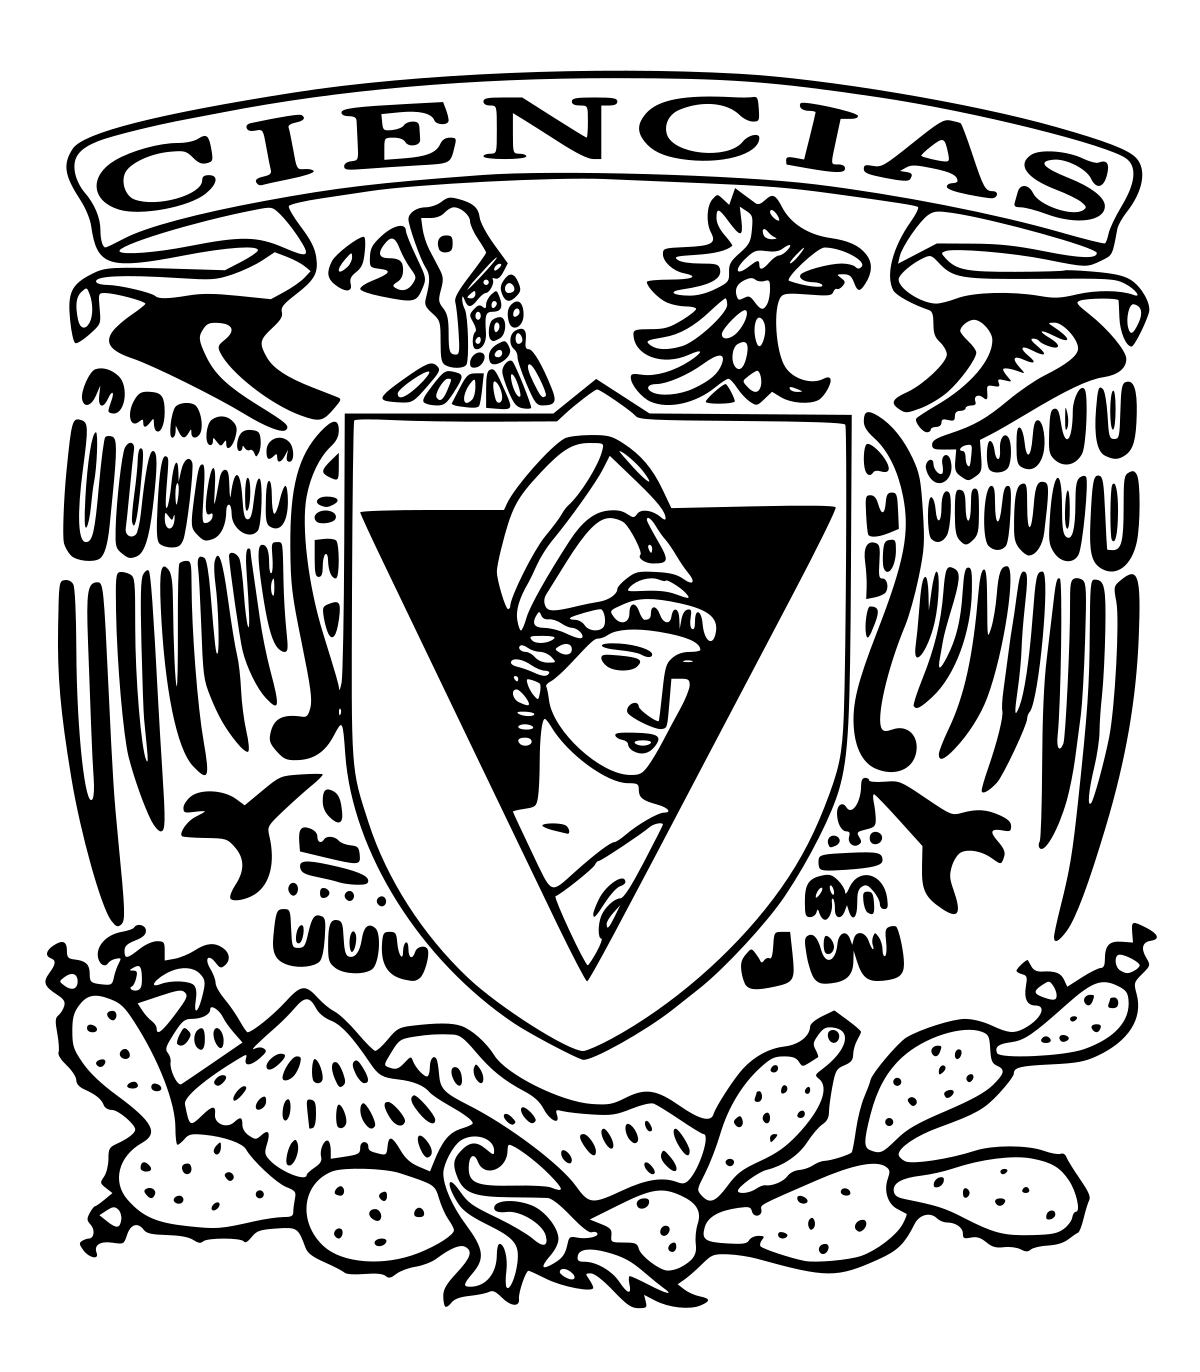
\includegraphics[width=0.8\linewidth]{imagenes/Logo_FC.png}
    \end{minipage}
    \vspace{3cm}
    \textbf{\large Practica 5}\\

    Licenciatura en Ciencias de la Computación\\
    Profesor: Gerardo Avilés Rosas \\
    \vspace{2cm}
    \textbf{Integrantes: }\\
    Cisneros Tenorio Diego Alexander\\
    Nuñez Ruiz José Manuel \\
    Olmos Ortiz Andrea Lucia\\
    Reynoso Ascencio Alexa \\
    Vega Navas Saúl \\
    \vspace{2cm}
    \textbf{Fecha de entrega: } 05 de octubre del 2026
    \vfill
\end{center}
\end{titlepage}
\tableofcontents
\newpage
\section{Restricciones de dominio de las tablas.}

\section*{Empleado}

\begin{longtable}{p{3.5cm} p{2.5cm} p{7.5cm} p{1.5cm}}
\label{tab:empleado}\\
\toprule
\textbf{Atributo} & \textbf{Tipo} & \textbf{Restricciones de dominio} & \textbf{Llave} \\
\midrule
\endfirsthead

\toprule
\textbf{Atributo} & \textbf{Tipo} & \textbf{Restricciones de dominio} & \textbf{Llave} \\
\midrule
\endhead
\bottomrule
\endfoot

CURP 
& varchar(18) 
& NOT NULL \newline CHECK(CHAR\_LENGTH(CURP) = 18)
& PK \\

FechaNacimiento 
& date 
& NOT NULL \newline CHECK(FechaNacimiento $\leq$ CURRENT\_DATE - INTERVAL '18 years')
& \\

Nombre 
& varchar(50)
& NOT NULL \newline CHECK(Nombre $<>$ '')
& \\

ApellidoPaterno 
& varchar(50) 
& NOT NULL \newline CHECK(ApellidoPaterno $<>$ '')
& \\

ApellidoMaterno 
& varchar(50) 
& NOT NULL \newline CHECK(ApellidoMaterno $<>$ '')
& \\

RFC 
& varchar(13) 
& NOT NULL \newline CHECK(RFC $<>$ '') \newline CHECK(CHAR\_LENGTH(RFC) = 13)
& \\

tipoEmpleado
& int
& NOT NULL \newline CHECK(tipoEmpleado $\geq$ 0 AND tipoEmpleado $\leq$ 3)
& \\

\end{longtable}

\vspace{2pt}
\textbf{Llave primaria:} CURP\\


\section*{Juego}

\begin{longtable}{p{3.5cm} p{2.5cm} p{7.5cm} p{1.5cm}}
\label{tab:juego}\\
\toprule
\textbf{Atributo} & \textbf{Tipo} & \textbf{Restricciones de dominio} & \textbf{Llave} \\
\midrule
\endfirsthead

\toprule
\textbf{Atributo} & \textbf{Tipo} & \textbf{Restricciones de dominio} & \textbf{Llave} \\
\midrule
\endhead

\bottomrule
\endfoot

idJuego 
& SERIAL4
& NOT NULL \newline CHECK(idJuego $>$ 0)
& PK \\

Nombre 
& varchar(50)
& NOT NULL \newline CHECK(Nombre $<>$ '')
& \\

Costo 
& int
& NOT NULL \newline CHECK(Costo $>$ 0 AND Costo \% 10 = 0)
& \\

Categoria 
& int
& NOT NULL \newline CHECK(Categoria $\geq$ 0 AND Categoria $\leq$ 3)
& \\

\end{longtable}

\vspace{2pt}
\textbf{Llave primaria:} idJuego\\

\section*{CorreoEmpleado}

\begin{longtable}{p{3.5cm} p{2.5cm} p{7.5cm} p{1.5cm}}
\label{tab:correoempleado}\\
\toprule
\textbf{Atributo} & \textbf{Tipo} & \textbf{Restricciones de dominio} & \textbf{Llave} \\
\midrule
\endfirsthead

\toprule
\textbf{Atributo} & \textbf{Tipo} & \textbf{Restricciones de dominio} & \textbf{Llave} \\
\midrule
\endhead

\bottomrule
\endfoot

CURP 
& varchar(18) 
& NOT NULL
& PK, FK \\

Correo 
& varchar(100) 
& NOT NULL
& PK \\

\end{longtable}

\vspace{2pt}
\textbf{Llave primaria compuesta:} CURP, Correo\\
\textbf{Llave foránea:} CURP $\rightarrow$ Empleado (CURP)\\


\section*{TelefonoEmpleado}

\begin{longtable}{p{3.5cm} p{2.5cm} p{7.5cm} p{1.5cm}}
\label{tab:telefonoempleado}\\
\toprule
\textbf{Atributo} & \textbf{Tipo} & \textbf{Restricciones de dominio} & \textbf{Llave} \\
\midrule
\endfirsthead

\toprule
\textbf{Atributo} & \textbf{Tipo} & \textbf{Restricciones de dominio} & \textbf{Llave} \\
\midrule
\endhead

\bottomrule
\endfoot

CURP 
& varchar(18) 
& NOT NULL
& PK, FK \\

Telefono 
& varchar(10) 
& NOT NULL
& PK \\

\end{longtable}

\vspace{2pt}
\textbf{Llave primaria compuesta:} CURP, Telefono\\
\textbf{Llave foránea:} CURP $\rightarrow$ Empleado (CURP)\\

\section*{Disparos}

\begin{longtable}{p{3.5cm} p{2.5cm} p{7.5cm} p{1.5cm}}
\label{tab:disparos}\\
\toprule
\textbf{Atributo} & \textbf{Tipo} & \textbf{Restricciones de dominio} & \textbf{Llave} \\
\midrule
\endfirsthead

\toprule
\textbf{Atributo} & \textbf{Tipo} & \textbf{Restricciones de dominio} & \textbf{Llave} \\
\midrule
\endhead

\bottomrule
\endfoot

idJuego 
& int 
& NOT NULL \newline CHECK(idJuego $>$ 0)
& PK \\

PuntosPorAcierto 
& int
& NOT NULL \newline CHECK(PuntosPorAcierto = 1)
& \\

\end{longtable}

\vspace{2pt}
\textbf{Llave primaria:} idJuego\\


\section*{Destreza}

\begin{longtable}{p{3.5cm} p{2.5cm} p{7.5cm} p{1.5cm}}
\label{tab:destreza}\\
\toprule
\textbf{Atributo} & \textbf{Tipo} & \textbf{Restricciones de dominio} & \textbf{Llave} \\
\midrule
\endfirsthead

\toprule
\textbf{Atributo} & \textbf{Tipo} & \textbf{Restricciones de dominio} & \textbf{Llave} \\
\midrule
\endhead

\bottomrule
\endfoot

idJuego 
& int 
& NOT NULL \newline CHECK(idJuego $>$ 0)
& PK \\

PuntosPorAcierto 
& int
& NOT NULL \newline CHECK(PuntosPorAcierto = 1)
& \\

\end{longtable}

\vspace{2pt}
\textbf{Llave primaria:} idJuego\\

\section*{Ritmo}

\begin{longtable}{p{3.5cm} p{2.5cm} p{7.5cm} p{1.5cm}}
\label{tab:ritmo}\\
\toprule
\textbf{Atributo} & \textbf{Tipo} & \textbf{Restricciones de dominio} & \textbf{Llave} \\
\midrule
\endfirsthead

\toprule
\textbf{Atributo} & \textbf{Tipo} & \textbf{Restricciones de dominio} & \textbf{Llave} \\
\midrule
\endhead

\bottomrule
\endfoot

idJuego 
& int
& NOT NULL \newline CHECK(idJuego $>$ 0)
& PK \\

PuntosTop5 
& int
& NOT NULL \newline CHECK(PuntosTop5 = 20)
& \\

\end{longtable}

\vspace{2pt}
\textbf{Llave primaria:} idJuego\\

\section*{Velocidad}

\begin{longtable}{p{3.5cm} p{2.5cm} p{7.5cm} p{1.5cm}}
\label{tab:velocidad}\\
\toprule
\textbf{Atributo} & \textbf{Tipo} & \textbf{Restricciones de dominio} & \textbf{Llave} \\
\midrule
\endfirsthead

\toprule
\textbf{Atributo} & \textbf{Tipo} & \textbf{Restricciones de dominio} & \textbf{Llave} \\
\midrule
\endhead

\bottomrule
\endfoot

idJuego 
& int
& NOT NULL \newline CHECK(idJuego $>$ 0)
& PK \\

PuntosTop5 
& int
& NOT NULL \newline CHECK(PuntosTop5 = 20)
& \\

\end{longtable}

\vspace{2pt}
\textbf{Llave primaria:} idJuego\\

\section{Restaurar backup de una BD en Docker}
Para la restauración del backup, se siguieron los pasos proporcionados en la practica.

\begin{enumerate}
    \item Revisión de los contenedores actuales.
    \begin{figure}[H]
    \centering
    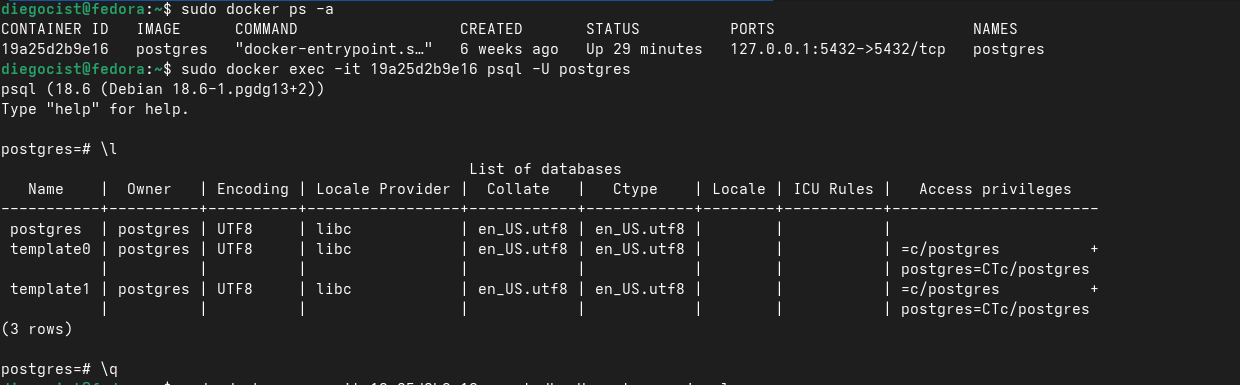
\includegraphics[width=0.5\textwidth]{imagenes/Diego-Revision.png}
    \end{figure}

    \item Se crea la base de datos ejemplo, se revisa que este vacía y se restaura el backup. En principio ocurre un error, pero fue solucionado al usar la instrucción pg\_restore.
    \begin{figure}[H]
    \centering
    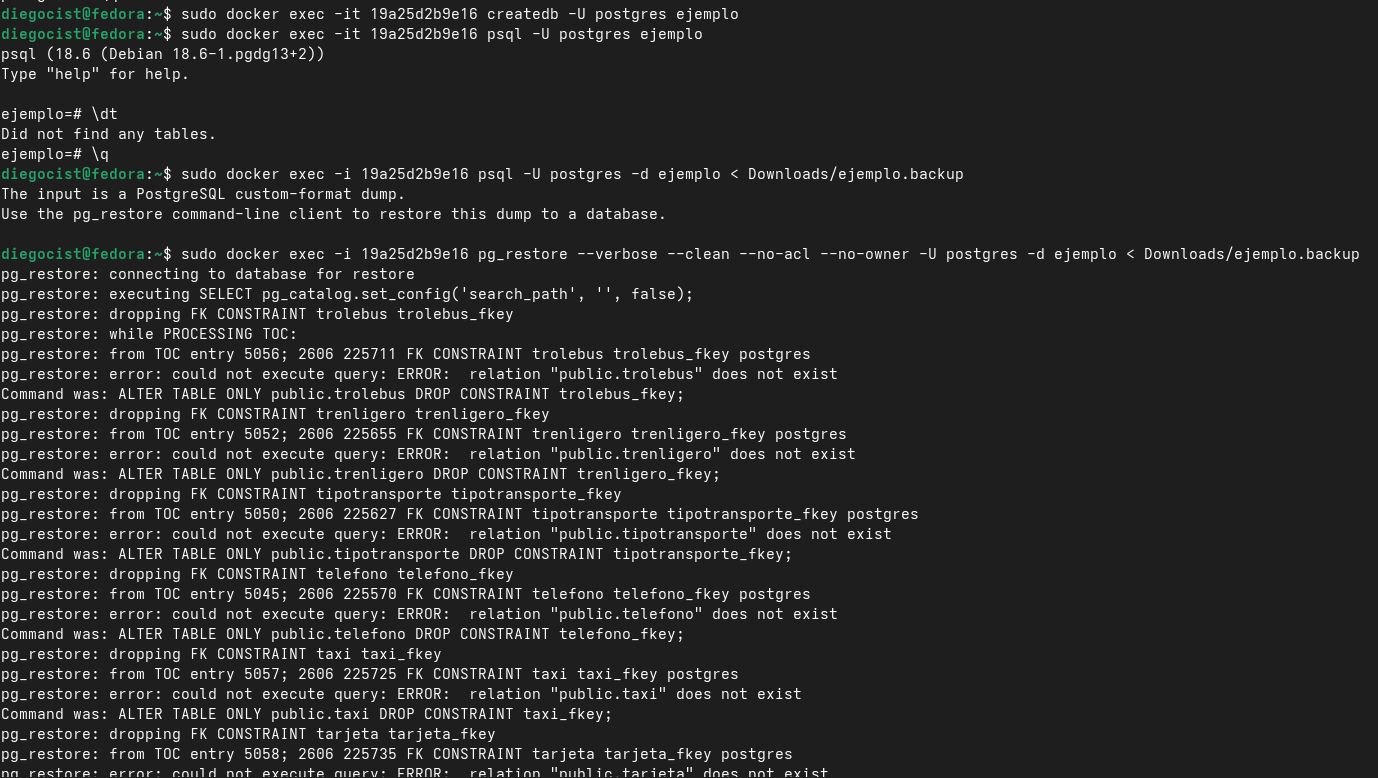
\includegraphics[width=0.5\textwidth]{imagenes/Diego-Restauracion.png}
    \end{figure}

    \item Revisión de las tablas en la base de datos.
    \begin{figure}[H]
    \centering
    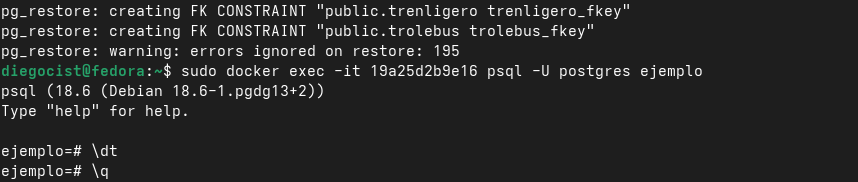
\includegraphics[width=0.5\textwidth]{imagenes/Diego-Tablas1.png}
    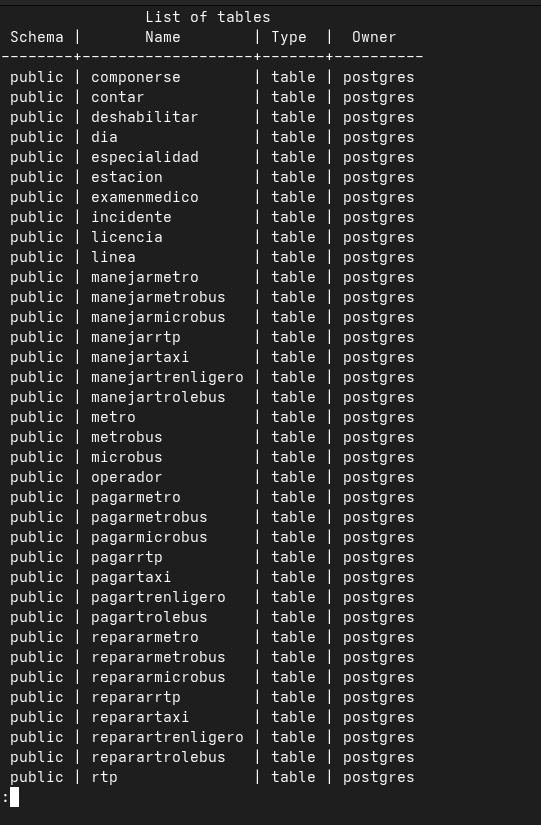
\includegraphics[width=0.5\textwidth]{imagenes/Diego-Tablas2.png}
    \end{figure}
\end{enumerate}


\end{document}
